%! TEX root = ../main.tex
\chapter{Propuesta de solución}
\label{chap:solucion}


\observacion{\textbf{Mirti}:
\begin{itemize}
\item Estructurar de nuevo el capítulo de solución 
\item Que se quiere hacer,
    que hay para hacer (herramientas), la solución en sí (más gráficos que
    explicaciones)
\item Grafo de dependencia de pasos (requisitos)
\item Disminuir texto
\item Elementos -> partes -> específico esc1 -> específico esc 2
    \item Imágenes con indicaciones
\item Que información se puede sacar de los logs
\item Poner por partes la conclusión
\item motor gráfico no es lo mismo motor de juegos
\item Punto medio para descripción de los motores (definir los criterios que
    todos deben tener)
\item Ver formato de la tabla comparativa
\end{itemize}
}

\observacion{Arturo:
\begin{itemize}
\item Decir que se quiere usar tecnologías móviles
\item Grafo de dependencias
\item No describir lo que se podría mostrar con una imagen
\item Mencionar partes del motor de videojuegos
\item Nuevo orden de caps:
    \begin{enumerate}
    \item Problema
    \item Requisitos o descripción (incluir retroalmientación)
        \begin{itemize}
        \item Que se quiere hacer
        \item Grafo de pasos
        \end{itemize}
    \item Motores y tecnologías
        \begin{itemize}
        \item motores (Descripción y comparación)
        \item Simulación (entidades, etc)
        \end{itemize}
    \item Solución
\end{enumerate}
\item Presentar para el lunes
    \begin{itemize}
        \item Introducción
        \item TICS
        \item Formato de impresión (a la derecha)
        \item Un capítulo siempre empieza en la página impar
    \end{itemize}
\end{itemize}}

\fixme{En el capitulo anterior, se describieron los fundamentos teóricos del uso de
    videojuegos serios en el ambiente educativo, dicha descripción se centra en
    aquellas áreas que requieren más practica para la adquisición de la pericia
    necesaria. Así, se identifico el área de enfermería como problemática, la
    formación de enfermeros y se selecciona algunos procedimientos que serán
    utilizados para el contenido de la solución}{}. A continuación se busca converger
todos los aspectos descriptos en capítulos anteriores.

La solución propuesta en este trabajo consiste en el desarrollo de una
aplicación para dispositivos móviles que se define como un juego serio llamado
\fixme{\Gls{yave}}{No es tarde para cambiar de nombre!}, basado en el
\fixme{construccionismo}{?}, el cual incluye conceptos de la gamificación, y de
simulación. El juego consiste en ofrecer a los usuarios, en este caso alumnos de
enfermería, un medio en el cual puedan realizar procedimientos de enfermería y
cuyo objetivo es servir como herramienta de apoyo en el aprendizaje.

\Gls{yave} permite al usuario poder seleccionar el procedimiento que quiera
realizar, dando la posibilidad de interactuar con un paciente y con una conjunto
de objetos que forman parte de las herramientas requeridas para realizar el
procedimiento seleccionado. Además, contempla la posibilidad de realizar
acciones relacionadas a la bioseguridad, y otros aspectos transversales a la
educación de un enfermero.

La solución no solo le permite al usuario realizar los procedimientos para
poner en practica sus conocimientos sobre el mismo, sino también evaluará al
usuario, dándole al final de cada sesión una puntuación y describiendo los
pasos realizados correcta e incorrectamente, proporcionando información acerca
de los puntos incorrectos.

%! TEX root = ../main.tex

\section{Arquitectura general}
\label{sec:solucion}

\observacion{Esta sección 7 deberá empezar con una descripción general (gráfico)
y debe ir explicando parte por parte}

A continuación se describe la arquitectura propuesta para la realización de una
juego serio, \fixme{se utiliza}{} la guía básica definida
por~\cite{pereira2009design} y descrita en~\ref{sec:desarrollo}.

Esta sección se enfoca en los aspectos técnicos de la creación del juego serio,
las competencias básicas relacionadas con la educación (segundo paso de la guía
descrita en~\ref{sec:desarrollo}) se definieron en las
secciones~\ref{sec:glasgow} y~\ref{sec:hemocultivo}.

La solución se basa en escena\fixme{s, u}{}na escena es un procedimiento definido
en~\ref{sec:seleccion_escenas}, cada escena tiene sus propias entidades, eventos
y requisitos específicos. \fixme{Adicionalmente existe otra escena denominada
Inicio que es la escena donde se inicia la solución.}{?}
%Inicio estaba en un \enquote

\observacion{Grafo de la arquitectura? Esta un poco desordenado}

Adicionalmente la solución cuenta con pantallas, que son vistas donde el usuario
puede seleccionar varias opciones, a continuación se describe el funcionamiento
global de la solución y la transición entre las escenas, pantallas y diversas
opciones existentes. Posteriormente se define como se interactúa con el entorno,
y a continuación se evalúa al alumno durante su experiencia con la solución.

\subsection{Flujo de la solución}

\observacion{Mejorar siguiente parrafo}
La solución consiste varios escenarios, y cada escenario, \fixme{existen}{Se
    presenta?} varias pantallas que muestran información relevante de acuerdo a
la situación de la simulación, la figura~\ref{fig:grafo_estados} es una
representación abstracta de este flujo de acciones disponibles dentro de la
solución.

\begin{figure}[H] 
\centering 
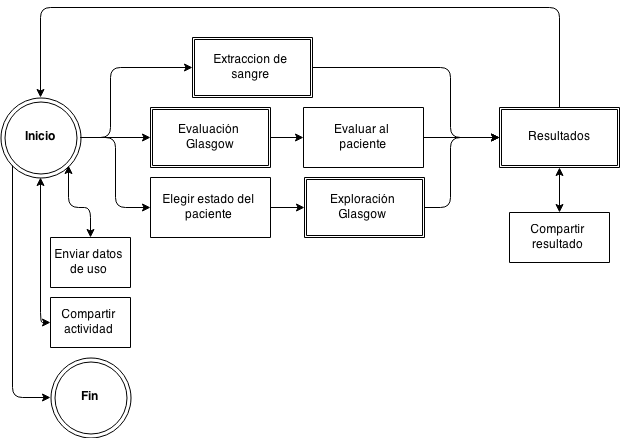
\includegraphics[scale=0.5]{solucion/images/grafo_escenas.png}
\caption{Diagrama de navegación entre los distintos escenarios y pantallas
    disponibles en la solución.}
\label{fig:grafo_estados}
\end{figure}

 
La figura~\ref{fig:grafo_estados} muestra que la solución empieza con una escena
denominada \emph{Inicio}. En la pantalla \emph{Inicio} se observa el escenario y 
opciones, que conducen a los escenarios \emph{Extracción de Sangre} y
\emph{Glasgow}. Otras opciones incluidos en el escenario \emph{Inicio} son
\begin{enumerate*}[label=\itshape\alph*\upshape)]
\item enviar datos de uso al \emph{backend},
\item iniciar sesión en el \emph{Facebook}, y,
\item salir de la simulación.
\end{enumerate*}


\fixme{El escenario \emph{Extracción de Sangre} finaliza al presionar la opción
\emph{Finalizar Partida} y luego se muestra la pantalla \emph{Resultados}, con
información de retroalimentación y la opciones de compartir resultado y volver
a la escena \emph{Inicio}.}{Finalizar }

Para iniciar el escenario \emph{Glasgow} existen dos caminos:
\begin{enumerate}
\item \textbf{Explorar}: desde la escena \emph{Inicio} se elige la opción \emph{Explorar
        Glasgow} en ese momento se muestra la pantalla \emph{Elegir estado del
        paciente}, donde se personaliza el estado del paciente y luego se inicia
    la escena. La escena finaliza con la opción \emph{Finalizar Partida} y se
    muestra la pantalla \emph{Resultados}.
\item \textbf{Evaluar}: desde la escena \emph{Inicio} se elige la opción \emph{Evaluar
        Glasgow} y se inicia la escena \emph{Glasgow} con un estado del paciente
    aleatorio.
    Al finalizar la escena, se muestra la pantalla \emph{Evaluar al paciente}
    donde se permite elegir el estado del paciente, y luego se pasa a la
    pantalla \emph{Resultados}
\end{enumerate}

Finalmente, en la pantalla \emph{Resultados} se permite compartir resultado y
volver a la escena \emph{Inicio}.

Todos los escenarios son utilizados de manera similar, la interacción con la
escena es siempre la misma.

\subsection{Transformaciones del punto de vista del usuario}

El usuario se desenvuelve en un entorno de tres dimensiones, en el cual realiza
las actividades relacionadas a la práctica, se distinguen dos tipos de acciones
principales que el usuario puede realizar:

\begin{itemize}
    \item \textbf{Alejamiento o acercamiento}: es el acto de acercar o alejar la
        cámara, y por consiguiente al usuario del paciente. Se realiza
        utilizando dos dedos, para realizar un acercamiento, mientras se
        mantiene presionada la pantalla con ambos dedos, se procede a alejar un
        dedo del otro, para realizar un alejamiento, se debe acercar ambos
        dedos.
    \item \textbf{Rotación}: se refiere al movimiento de rotación alrededor de
        un foco, que en ambas escenas es el paciente, para realizarla, se utiliza
        un dedo, y se mueve el dedo en cualquier dirección, la cámara, se moverá
        en la dirección contraria.
\end{itemize}

\subsection{Evaluación del usuario}
\label{sec:eca_impl}

\todo[backgroundcolor=white,inline,caption={Pregunta}]{Si esto esta flotando acá
    es por que no sabemos donde podemos poner los detalles de implementación del
    Motor, no se ponen en la parte de extracción de sangre para mantener la
    consistencia con glasgow.}

En la sección~\ref{sec:eca} se describen los \Gls{eca}, y los mismos son
utilizados para poder realizar la evaluación del alumno en la solución.

Definir si las acciones de un usuario son correctas utilizando un motor
\Gls{eca} es sencillo teniendo en cuenta que sólo se deben definir un
conjunto de acciones que se deben realizar, y agregar una acción que verifica si
los pasos realizados fueron los correctos.

Se describe como se crean las reglas, de manera a explicar como son utilizadas
para la evaluación de las acciones realizadas por el usuario.

La definición de las reglas se realiza de la siguiente forma:

\begin{algorithm}[H]
\caption{Creación de regla de verificación de calzado de guantes}
\label{alg:rule_guante}
\lstset{style=sharpc}
\begin{lstlisting}
Rule.New().
     When(``enfermero.guantes.calzar'').
     Then(enviroment => enviroment.
            estadoPaciente.TieneManosLimpias()).
\end{lstlisting}
\end{algorithm}

La regla del algoritmo~\ref{alg:rule_guante} controla que el estudiante ha
realizado la acción \enquote{Calzarse los guantes}, y en ese momento tenga las
manos limpias.

\subsubsection{Estados de una regla}
\observacion{Hacer referencia a la figura 7.2 o mover adelante (la figura del
    ciclo de vida)}

Una regla puede estar en uno de los siguientes estados:

\begin{enumerate}
\item \textbf{BEGIN} Es una regla que recién fue creada, no realiza ninguna
	acción.
\item \textbf{WAITING\_FOR\_RULE:} Es un estado en el que esta esperando que otras reglas
	sean lanzadas. En este estado, es un suscriptor de las reglas por la que
	espera, y no forma parte del ciclo de ejecución del motor de reglas.
\item \textbf{WAITING\_FOR\_EVENT:} Es un estado en el que esta escuchando que sean
	lanzados los eventos a los que escucha, este es el estado principal. En
	este estado, es un suscriptor de los eventos por los que espera, y no
	forma parte del ciclo de ejecución del motor de reglas.
\item \textbf{WAITING\_FOR\_CONDITION:} La regla ya no espera por ningún evento y las
	reglas de las que depende ya han sido lanzadas, se verifica cada cierto
	tiempo si el entorno cumple con una condición definida. 
\item \textbf{FINISH:} Estado final de una regla.
\end{enumerate}

\begin{figure}
\centering
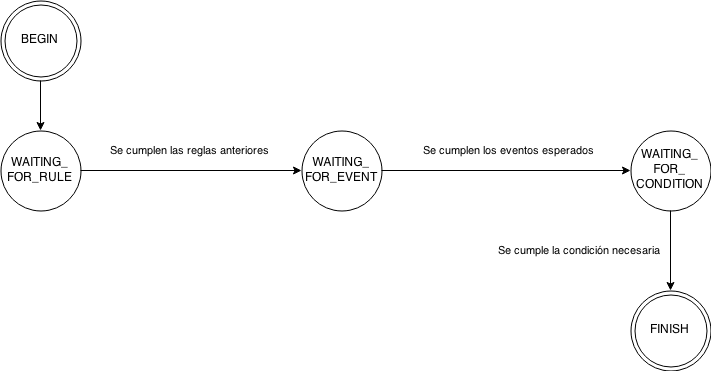
\includegraphics[width=12cm]{solucion/images/rules_flow.png}
\caption{Ciclo de vida de una regla}
\label{fig:rule_flow}
\end{figure}

En la figura~\ref{fig:rule_flow} se observa la evolución de una regla, es
importante notar que una regla solo puede avanzar en este flujo.

\subsubsection{Motor de ejecución}

Un motor de reglas \gls{eca}, requiere de un proceso que evalúe constantemente
las reglas para verificar si las mismas deben ser lanzadas o
no\cite{bailey2004event,galton2002two}, un algoritmo comúnmente utilizado para
realizar la verificación es el algoritmo de \enquote{RETE}\revisar{Tener el
    algoritmo en la presentación, como anexo}\cite{de2001eca}, la cantidad de
reglas definidas, y la no dependencia circular entre ellas, hace innecesario la
implementación de tal algoritmo\cite{de2001eca}. 

De acuerdo a la descripción dada en~\ref{sec:eca_ejecucion}, la propuesta
implementada utiliza una ejecución inmediata, principalmente por la sencillez
de las reglas, es decir, las reglas no realizan un proceso complejo, solamente
controlan el estado del entorno y lo validan.

Además, la ejecución inmediata es importante por que el entorno no sufre
modificaciones entre el evento lanzado y la ejecución de la regla, según
\cite{bailey2004event}, este es el factor más importante para determinar el tipo
de ejecución deseado.

El motor de reglas actúa sobre aquellas reglas en estado
\emph{WAITING\_FOR\_CONDITION} e invoca al procedimiento que se encarga de
validar si la regla puede ser activada (el procedimiento es único por cada
regla), si el mismo determina que la regla puede ser lanzada, el motor ejecuta
la acción de la regla y modifica el estado de la regla a \emph{FINISH}.

%A continuación, se describen todos los escenarios, primeramente se da una
%descripción general de los escenarios y se procede a explicar los detalles de
%los mismos, incluyendo las entidades, eventos y acciones que pueden ser
%realizados en el mismo.

\section{Inconvenientes de diseño}

Los mayores inconvenientes de diseño de la aplicación se dieron en el momento de
validar tanto el contenido de la aplicación como la interfaz de usuario, para
sobrellevar estos inconvenientes fueron requeridos la intervención de terceros.

A continuación se explica en detalle cada uno de los casos.

\subsection{Interfaz de usuario}

Como parte del diseño y desarrollo de la solución se realizó una prueba de
interfaz de usuario con alumnos de la carrera de Ingeniería en Informática de la
\Gls{fpuna}, estas pruebas fueron realizadas con personas que están
acostumbradas al uso de interfaces similares y que, de hecho pueden ser mas
criticas a la hora de evaluarlas. Esta prueba se explica en detalle en el
capítulo~\ref{chap:evaluacion} y los resultados en el
capítulo~\ref{chap:analisis}.

Principalmente son dos las cualidades de una interfaz gráfica que se pueden
someter a prueba: la funcionalidad y la usabilidad. Con la primera se pretende
responder preguntas como \textit{¿Se puede usar cierta función?},
\textit{¿Funciona como se espera?}, o \textit{¿Es correcta?}; y con respecto a
al usabilidad, se espera poder responder a \textit{¿Puede el usuario
    utilizar fácilmente la función?}, o \textit{¿Su uso es intuitivo y fácil de
    aprender?}\cite{fragaverificacion}.

Las pruebas de interfaces de usuario ayudan a que los usuarios puedan
concentrarse mas en el problema en vez de poner los esfuerzos en recordar todas
las opciones que ofrece la solución que se utiliza para resolver el
problema\cite{horowitz1993graphical}.

Luego de las pruebas de interfaz de usuario, se hicieron correcciones a los
problemas encontrados en la interfaz, los mayores inconvenientes fueron con
respecto a la usabilidad y la interacción tanto con el entorno como con los
objetos dentro de la simulación. Estas correcciones, como paso posterior, fueron
probadas por profesores de la carrera de enfermería del \Gls{iab} los cuales
dieron su visto bueno.

Otra de las razones por las cual la prueba fue realizada con alumnos que no
formaban parte de la población a la que iba dirigida la aplicación, es la poco
disponibilidad de tiempo con la que cuentan los alumnos de enfermería y mas aún
los profesionales que están encargados de su aprendizaje.

\subsection{Validaciones de contenido}

Llamamos validación de la simulación o la aplicación desarrollada al hecho de
que el contenido de la misma sea correcto y además que la forma de realizar o
representar dicho procedimiento este acorde al mismo. Este tipo de validaciones
fueron realizadas reiteradamente en reuniones con distintos profesores de la
carrera de enfermería del \Gls{iab}.

Cada corrección solicitada fue evaluada y aprobada posteriormente por los
mismos. Como validación final la aplicación fue presentada en totalidad frente a
un plenario de cuatro profesores del instituto.

El mayor inconveniente en cuanto a las validaciones fueron la forma de
representación tanto de la información como de la simulación de objetos.

\section{Backend de la solución}
\observacion{Podrían explicar que hacen con estos datos, no listar resultados de
    queries, pero sí explicar que tipo de información esperan obtener con esta
    concretamente. Para qué?, Por qué?, intro a análisis}

La solución almacena información detallada acerca de las acciones del usuario,
las condiciones de estas acciones y el contexto en el cual fueron ejecutadas.

Esta información es almacenada en un servidor dedicado para su posterior
análisis.

\begin{figure}[ht]
\centering
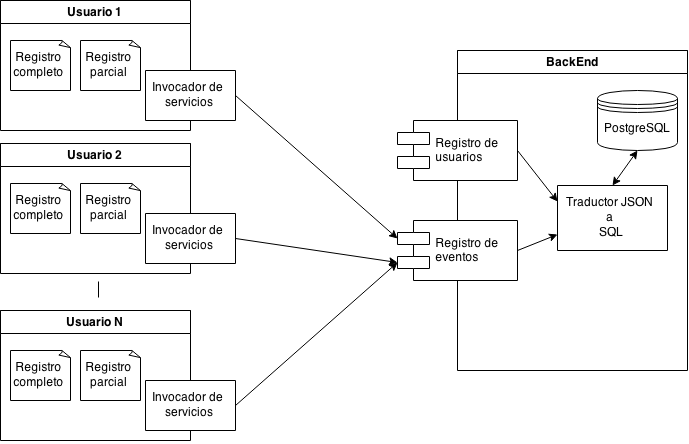
\includegraphics[scale=0.5]{solucion/images/backend_diagrama.png}
\caption{Diagrama de la interacción de los usuarios con el \textit{BackEnd}, se
    puede observar a grandes rasgos, los componentes del sistema y los servicios
    que ofrece.}
\label{fig:backend_diagrama2}
\end{figure}

En la figura~\ref{fig:backend_diagrama} se pueden observar los componentes
principales de este sistema, y su interacción con los dispositivos móviles de
los usuarios. 

\subsection{Registro de usuarios}

Para poder determinar a qué usuario corresponde qué conjunto de datos, durante la
instalación de la solución en los dispositivos móviles de los usuarios, se ingresa como
un dato adicional el número de teléfono del mismo, estos datos se registran
en el \textit{BackEnd} al mismo tiempo en el que se muestra la solución al usuario.

De esta forma, en el sistema se encuentran los datos proveídos por la
simulación, así como el nombre del usuario. Es necesario almacenar el nombre del
usuario para las diversas encuestas que se realizan (las encuestas para alumnos
que participaron en el experimento no son anónimas), de esta manera se puede
saber, dada una encuesta, a que alumno corresponde y el uso que le dio a la
solución. Estas encuestas son explicadas en detalle en~\ref{chap:evaluacion} y sus 
resultados en~\ref{chap:analisis}.

\subsection{Registro de eventos}

Las acciones que realiza el usuario son almacenadas en un archivo temporal,
dentro del dispositivo móvil del usuario, cuando este decide enviar la
información, estos datos se transmiten por la red a un servidor que almacena el
\textit{BackEnd}.

Una vez que el usuario envía sus datos de uso, el archivo de registros
local se limpia, permitiendo así que nuevos registros sean añadidos.
Adicionalmente, existe un archivo de respaldo, que contiene toda la información
que se registró del usuario, incluyendo aquellas que ya fueron enviadas al
servidor \textit{BackEnd}.

\subsection{Detalles de implementación}

El \textit{BackEnd} es un sistema web, desarrollado en \textit{Java}, y
desplegado en un servicio \textit{OpenShift}, el cual está disponible $24$ horas
al día, los $7$ días a la semana, asegurando así, que cuando el usuario desee
enviar datos lo pueda hacer sin problemas.

El sistema tiene dos servicios web que permiten el registro de usuarios y el
registro de eventos, ambos reciben una lista de elementos y los almacenan en una
base de datos \textit{PostgreSQL}.

Estos dos servicios implementan un mecanismo de seguridad sencillo, basado en usuario y
contraseña, el único objetivo de este mecanismo, es que los datos no sean
fácilmente accesibles, pues contienen datos sensibles.

La petición enviada desde la solución, contiene el número de teléfono del
usuario, un identificador único generado por \textit{Unity3D} y una lista de
eventos, en formato \Gls{json}.




%%% SOLUCION
% 1.1. Solución
% 1.1.1. Partes de la simulación
% 1.1.2. Grafo de estados
% 1.1.3. Inicio
% 1.1.4. Extracción de muestras de sangre
% 1.1.5. Valoración de la escala de Glasgow
% 1.1.6. Pantalla de resultados
% 1.2. Inconvenientes de diseño
% 1.2.1. Interfaz de usuario
% 1.2.2. Validaciones de contenido
% 1.3. Backend de la solución
% 1.3.1. Registro de usuarios
% 1.3.2. Registro de eventos
% 1.3.3. Detalles de implementación


%%%% PROPUESTA DE TINCHO
% 1. Arquitectura general
%       Grafo de estados
%       Partes de la simulación (eventos, entidades, etc)
%       Motor achicamos los suficiente, puede ser un \subsubsection
% 2. Interfaz
%       Inicio
%       Hemocultivo
%           Pantalla de resultados
%       Glasgow
%           Pantalla de resultados
% X.    Inconvenientes de diseño
%           Interfaz de usuario
%           Validaciones de contenido
% 3. Backend
%       Registro de usuarios
%       Registro de eventos
%       Detalles de implementación
